\documentclass{standalone}
\usepackage{fontspec}
\setsansfont{DejaVuSans.ttf}[Path=./,Kerning=Off,Ligatures={TeXOff,NoCommon}]
\usepackage{tikz}
\begin{document}
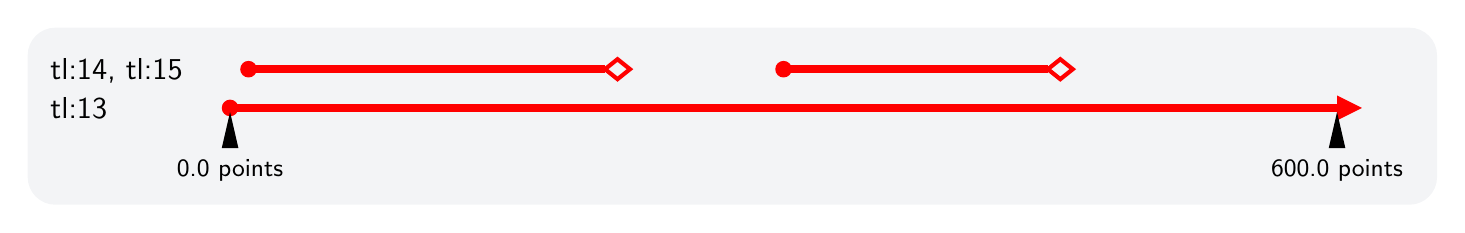
\begin{tikzpicture}[x=1pt,y=1pt,miter limit=4,font=\sffamily]
\definecolor{ts000000}{HTML}{000000}
\definecolor{tsF3F4F6}{HTML}{F3F4F6}
\definecolor{tsFF0000}{HTML}{FF0000}
\begin{scope}[shift={(16,16)}]
\path[rounded corners=10pt,fill=tsF3F4F6] (0,0) rectangle (509.2715,63.9766);
\path[draw=tsFF0000,line width=3pt] (73.1377,34.9766) -- (473.1377,34.9766);
\path[fill=tsFF0000] (73.1377,34.9766) circle[radius=3];
\path[fill=tsFF0000] (482.1377,34.9766) -- (473.1377,39.4766) -- (473.1377,30.4766) -- cycle;
\path[draw=tsFF0000,line width=3pt] (79.8044,48.9766) -- (208.6377,48.9766);
\path[fill=tsFF0000] (79.8044,48.9766) circle[radius=3];
\path[draw=tsFF0000,line width=1.5pt] (208.6377,48.9766) -- (213.1377,52.5766) -- (217.6377,48.9766) -- (213.1377,45.3766) -- cycle;
\path[draw=tsFF0000,line width=3pt] (273.1377,48.9766) -- (368.6377,48.9766);
\path[fill=tsFF0000] (273.1377,48.9766) circle[radius=3];
\path[draw=tsFF0000,line width=1.5pt] (368.6377,48.9766) -- (373.1377,52.5766) -- (377.6377,48.9766) -- (373.1377,45.3766) -- cycle;
\path[fill=ts000000] (73.1377,33.4766) -- (70.1377,20.4766) -- (76.1377,20.4766) -- cycle;
\path[fill=ts000000] (473.1377,33.4766) -- (470.1377,20.4766) -- (476.1377,20.4766) -- cycle;
\node[anchor=base west,inner sep=0,font=\sffamily\fontsize{11}{12.8047}\selectfont,text=ts000000] at (8,45.1685) {tl:14, tl:15};
\node[anchor=base west,inner sep=0,font=\sffamily\fontsize{11}{12.8047}\selectfont,text=ts000000] at (8,31.1685) {tl:13};
\node[anchor=base,inner sep=0,font=\sffamily\fontsize{9}{10.4766}\selectfont,text=ts000000] at (73.1377,10.1226) {0.0 points};
\node[anchor=base,inner sep=0,font=\sffamily\fontsize{9}{10.4766}\selectfont,text=ts000000] at (473.1377,10.1226) {600.0 points};
\end{scope}
\end{tikzpicture}
\end{document}
